% conventrion problem
% redo, undo: hooks, history
% dawing tool!

Graphical content is the most efficient and intuitive way to deliver the explanation of an answer to other users comparing with pure textual content. In this section, Choices for graphical technologies on the Web will be analysed in order to figure out which is the ideal and fit the graphical discussion system most. And a feasible approach of storing graphical data will be proposed. At last, a drawing tool will also be designed to offer user interfaces for drawing elements on the drawing board.

\subsection{Canvas over SVG}
It seems that both Canvas and SVG are good candidates as a graphic technology for the graphic discussion system. Both of them provides native methods to render rich varieties of elements like path, circle, rectangle and so on. Which would be a better choice above the context of discussion system, should be analysed at first.

\subsubsection{Efficiency}
As mentioned in section \ref{graphics-section}, the rendering efficiency is the primary deficiency happening to SVG. 

And graphic technologies are not only simply used for rendering a static graphical content in the system. Dragging, resizing or deleting an element are the basic features of a drawing tool, which provides input of graphical content. All these features are only able to be accomplished by re-rendering the elements on the drawing board. 

Considering that all contributions in the system are made with graphical contents, efficiency plays a significant role especially on mobile devices with old hardware. Choosing Canvas will give users better usability while viewing the contributions as well as using the efficient drawing tool without janky feeling. 

\subsubsection{Extensibility}
% WebGL for further usage, animation support?
TDB

\subsection{Storable and Reversible Canvas Data }

A focus point in the thesis is how to store the graphical content submitted by users. In the traditional way, graphical data could only be stored either in file system or in the database with encoded format, for example Base64 encoded images. 

\subsubsection{Deficiency of Canvas - Storable Image Data}
Canvas provides a native method called \textit{getImageData()} to export the whole Canvas context including the size of Canvas and pixels on Canvas to an image data. The image data exported by canvas represents the underlying pixel data with the format of \textit{Uint8ClampedArray}. The \textit{Uint8ClampedArray} typed array represents an array of 8-bit unsigned integers clamped to 0-255 [reference], which implies the position of the pixel as the index of array and the color of pixel as value from 0 to 255. A example is taken in figure \ref{fig:canvas-imagedata} shows a Canvas with content and its simplified ImageData. 

\begin{figure}[!htbp]
  \centering
    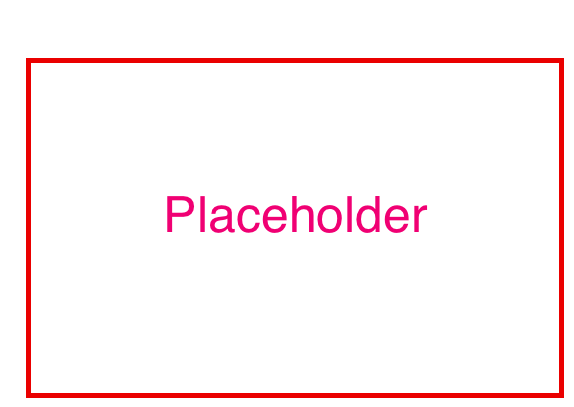
\includegraphics[width=0.6\textwidth]{Figures/placeholder.png}
  \caption{placeholder}
  \label{fig:canvas-imagedata}
\end{figure}

Restoring with the exported ImageData is also possible in Canvas by using its native method called \textit{putImageData()}. Basically, the concept of \textit{putImageData()} is traversing the ImageData exported by Canvas, and re-drawing each pixel at the position according to the index in the \textit{Uint8ClampedArray} and applying the color to the pixel based on the value from 0 to 255 stored in the array.

Natively exported result of image data could basically meet the storing demand, however, the data redundancy in the native exported format representing the properties of each pixel is still very huge. Storing such kind of data will cause high demand on storage space when plenty of graphical contributions are made in there system.

Additionally, it is expected that users are able to remove, resize and modify the elements in the canvas while quoting others' contributions. However, natively exported result of image data could only describe each pixel but not each element on the Canvas, which means modification on the elements is not possible even though the whole canvas could be reproduced with graphical content by others. 

Therefore, a workable solution should be concepted and new data model describing the graphical content in Canvas should be designed to meet the demands mentioned above.

\subsubsection{Solution - Objectification of Elements in Canvas}

Even though Canvas has native methods to draw different shapes of elements, but Canvas only render them pixel by pixel, it knows nothing of the shapes that are drawn. Therefore, removal or modification of a already drawn element is not possible. In this condition, a feasible solution is to wrap the Canvas and objectify the original elements which could be stored and persisted in a stack. Furthermore, the wrapper on Canvas should also provide methods to render, modify, remove the custom elements. 

The general conception of the wrapped Canvas is illustrated in figure \ref{fig:wrapped-canvas}.

\begin{figure}[!htbp]
  \centering
    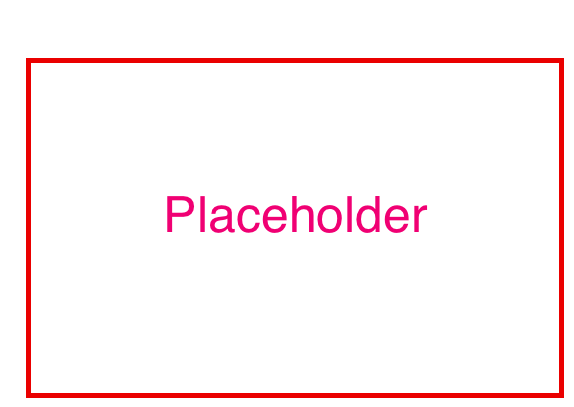
\includegraphics[width=0.6\textwidth]{Figures/placeholder.png}
  \caption{placeholder}
  \label{fig:wrapped-canvas}
\end{figure}
% wrapped canvas, multiple shapes, modify -> rerender.
The wrapped Canvas has a list of objectified elements which are visible on Canvas. Now there are new definitions for rendering, modification of an objectified element:
\begin{itemize}
\item
\textbf{Rendering Canvas}: the list of elements maintained by wrapped Canvas will be traversed and each element will be rendered by calling the native drawing method of Canvas. Position and style of the element in Canvas refer to the properties of its object.  
\item
\textbf{Modification or Removal}: In case the methods for modifying or removing provided by element object in wrapped Canvas are fired, the whole Canvas will be re-rendered in the same way of rendering the Canvas initially.

\end{itemize}
Now rendering means that the list of elements maintained by wrapped canvas is traversed and each elements are 

\subsubsection{Data Model Exported By Wrapped Canvas}
Since the wrapped Canvas maintains a list of objects for elements, which also contain the properties such as position, color, size and so on, so the exporting of image data is now really simple. A composition of all objectified elements' properties is already enough to describe the whole canvas. Figure \ref{fig:wrapped-canvas-data} reveals the approach and data model output from wrapped 
canvas.

\begin{figure}[!htbp]
  \centering
    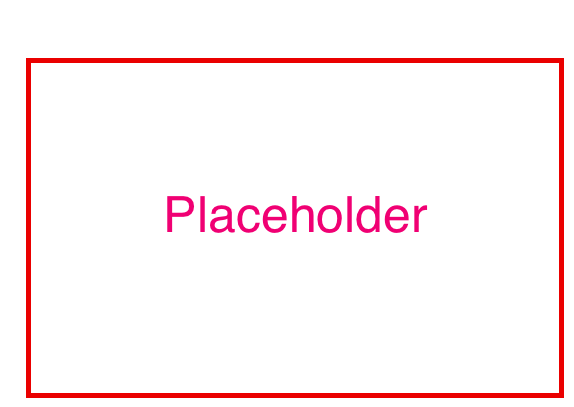
\includegraphics[width=0.6\textwidth]{Figures/placeholder.png}
  \caption{placeholder}
  \label{fig:wrapped-canvas-data}
\end{figure}
% properties on objectified elements, -> data model (json) -> restore from data.

After converting all elements in wrapped canvas, the new data model is much more efficient for storing comparing to the raw image data. The wrapped Canvas will also provides a method to restore the output data, create new objectified elements by giving the properties of the data model, and re-render the elements into original Canvas pixel by pixel. With this approach, the feature of modification on elements while quoting other contributions could also be achieved. 

\subsection{Drawing Tool}

After the conception of a feasible wrapped canvas as base of the container for all elements, a drawing tool which provides user interfaces to draw variable shapes as well as texts should be designed in the next step. 

First of all, user interfaces for selecting different drawing mode like drawing circle, rectangle or line should be designed. Buttons for toggling various drawing modes are the best choice in this case.

Because drawing elements in different shapes has distinct behaviors, so listeners for each specific drawing mode should be defined. When the button for toggling drawing mode is clicked by user and specific drawing mode is activated, the correlative listener will be initiated. Clicking events or moving events of the mouse on Canvas will be captured and processed. Meanwhile, drawing behaviors are also performed according the mouse events fired by user.

\begin{figure}[!htbp]
  \centering
    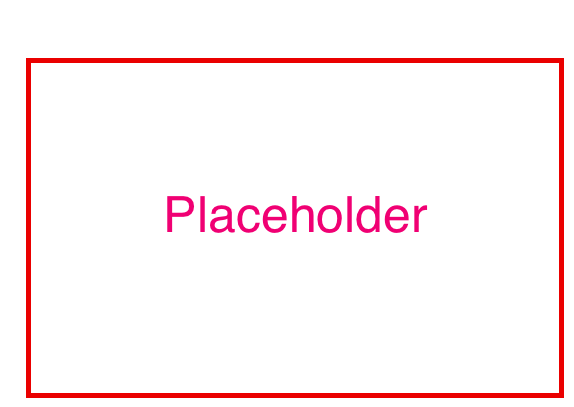
\includegraphics[width=0.6\textwidth]{Figures/placeholder.png}
  \caption{placeholder}
  \label{fig:drawing-tool-concept}
\end{figure}
% drawing tool, with diff drawing mode, start listener, stop old listener (life cycle).

Figure \ref{fig:drawing-tool-concept} illustrated the conception of drawing tool with user interfaces and life cycle of event listeners for each drawing mode.